\documentclass[a4paper, 11pt]{article}
\usepackage[italian]{babel}
\usepackage[utf8]{inputenc}
\usepackage{amsmath}
\usepackage{imakeidx}
\usepackage{amsfonts}
\usepackage{amssymb}
\usepackage{float}
\usepackage{graphicx}
\usepackage{caption}
\usepackage[paper=a4paper]{geometry}
\usepackage[shortlabels]{enumitem}
\usepackage{hyperref}
\usepackage{caption}
\captionsetup[figure]{justification=centering}
% Frontespizio config
\usepackage[nowrite]{front-th}
\usepackage{pdfpages}
\usepackage{caption}
\captionsetup[figure]{justification=justified}

\usepackage{fancyhdr} % <-- aggiunto
\pagestyle{fancy}     % <-- imposto lo stile fancy
\setlength{\headheight}{32.5316pt}
\addtolength{\topmargin}{-20.5316pt}
\fancyhf{}
\rhead{\includegraphics[width=1cm]{Immagini_EX/Logo_Università_di_Udine.png}} % <-- logo in alto a destra
\hypersetup{
    colorlinks,
    citecolor=black,
    filecolor=black,
    linkcolor=black,
    urlcolor=black
}

\setcounter{secnumdepth}{4}
\setcounter{tocdepth}{4}

% --- INIZIO SOSTITUZIONE MINTED CON LISTINGS ---
\usepackage{listings}
\usepackage{xcolor} % Necessario per definire i colori

\definecolor{codegray}{gray}{0.95}
\definecolor{codegreen}{rgb}{0.0, 0.5, 0.0} % Per i commenti
\definecolor{codered}{rgb}{0.9, 0.0, 0.0}   % Per le stringhe
\definecolor{codeblue}{rgb}{0.0, 0.0, 0.9}   % Per le parole chiave

\lstdefinestyle{mycodestyle}{
    backgroundcolor=\color{codegray}, % Colore di sfondo
    basicstyle=\small\ttfamily,       % Stile del testo del codice (dimensione piccola, font a spaziatura fissa)
    breaklines=true,                  % Permette al codice di andare a capo
    frame=single,                     % Aggiunge un bordo singolo
    framesep=5pt,                     % Spazio tra il bordo e il codice
    framerule=0.5pt,                  % Spessore del bordo
    rulecolor=\color{orange!70},     % Colore del bordo (arancione come nel tuo esempio)
    numbers=left,                     % Numerazione delle righe a sinistra
    numberstyle=\tiny\color{gray},    % Stile dei numeri di riga
    stepnumber=1,                     % Incremento dei numeri di riga
    numbersep=8pt,                    % Spazio tra numeri e codice
    showspaces=false,                 % Non mostrare spazi come simboli
    showtabs=false,                   % Non mostrare tab come simboli
    showstringspaces=false,           % Non mostrare spazi nelle stringhe
    commentstyle=\color{codegreen}\textit, % Stile per i commenti (verde, corsivo)
    keywordstyle=\color{codeblue}\bfseries, % Stile per le parole chiave (blu, grassetto)
    stringstyle=\color{codered},      % Stile per le stringhe (rosso)
    % Se vuoi un titolo/didascalia per il blocco di codice, potresti usare captionpos, ad esempio:
    % captionpos=b, % didascalia sotto
    % caption={Descrizione del codice},
}
% --- FINE SOSTITUZIONE MINTED CON LISTINGS ---


\renewcommand{\contentsname}{Indice}

\newcommand{\myfrontpage}{%
  \begin{titlepage}
  \centering
  \preparefrontpage
  \end{titlepage}
  %\global\let\centering\relax % Disabilita centering globale
}

\fontoptionnormal

\makeatletter
\def\front@thecandidate{Candidato}
\def\front@thecandidates{Candidati}
\def\front@theadvisor{Relatore}
\def\front@theadvisors{Relatori}
\makeatother


% Dati frontespizio
\Universita{Udine}
\Logo[3.5cm]{./Immagini_EX/Logo_Università_di_Udine.png}
\Dipartimento{Scienze Matematiche, Informatiche e Fisiche}  % Aggiunto in sostituzione di Facoltà
\Corso[Laurea]{Internet Of Things, Big Data, Machine Learning}
\Annoaccademico{2024--2025}
\Titolo{Laboratorio di Algoritmi e Strutture Dati\bigbreak - \bigbreak Verifica della complessità asintotica degli algoritmi di ordinamento}
\Candidato{Andrea Gioia\\(169484) - 169484@spes.uniud.it}
\Candidato{Luca Gamberini\\(168712) - 168712@spes.uniud.it}
\Candidato{Kent Idrizi\\(168711) - 168711@spes.uniud.it}
\Relatore{Prof. Gabriele Puppis}
\Relatore{Prof. Carla Piazza}
% \Correlatore{Prof. Marco Sciandrone}  % Commentato come richiesto



\begin{document}
\myfrontpage

\thispagestyle{empty} 
%\preparefrontpage

\newpage

\tableofcontents
\newpage
\section{Introduzione}
Il progetto include le misurazioni e la conseguente graficazione di 4 algoritmi di ordinamento:
\begin{itemize}
    \item QuickSort
    \item QuickSort 3 Way
    \item CountingSort
    \item RadixSort
\end{itemize}
\subsection{Specifiche tecniche}
Le specifiche tecniche delle misurazioni sono state:
\begin{itemize}
    \item Array generato con valori decimali \textbf{casuali}
    \item La lunghezza dell'array è compresa tra 100 e 100 mila valori
    \item Il valore di ciascun elemento dell'array varia casualmente tra 10 e un milione
\end{itemize}
Gli algoritmi sono stati implementati in linguaggio \textbf{Python}. \\
Le misurazioni dei tempi sono state acquisite tramite la funzione \href{https://docs.python.org/3/library/time.html#time.perf_counter}{\textit{\texttt{perf\char`_counter}}} della libreria \textit{time}.

\section{Algoritmi}
Gli algoritmi di ordinamento presi in esame presentano caratteristiche differenti e risultano più o meno efficienti in base alle carattestiche dell'array di elementi da ordinare.

\subsection{QuickSort}
Algoritmo di ordinamento ricorsivo del tipo divide-et-impera, basato sulla suddivisione in \textit{n} sottoproblemi risolti ricorsivamente fino al raggiungimento del caso base.

Non presenta la necessità di utilizzo di strutture dati aggiuntive, di conseguenza lo scambio di elementi avviene in-place.

\noindent\textbf{Idea}

\begin{itemize}
  \item[\textit{Divide}:] Partizionamento dell'array $A[p:r]$ in due sottoarray $A[p:q-1]$ (parte inferiore) e $A[q+1:r]$ (parte superiore) in modo che ciascun elemento della parte inferiore sia minore o uguale al pivot $A[q]$, il quale è a sua volta minore o uguale a ciascun elemento della parte superiore. Calcolare l'indice $q$ del pivot fa parte della procedura di partition.
  
  \item[\textit{Impera}:] Richiamo ricorsivo di quicksort su ciascun sottoarray $A[p:q-1]$ e $A[q+1:r]$. Infine, per combinare, non serve fare nulla dato che i due sottoarray sono già ordinati, per cui l'intero sottoarray $A[p:r]$ risulta ordinato.
  
  \item La procedura Partition permette di stabilire un perno; a quel punto gli elementi precedenti sono minori del perno mentre quelli a destra sono maggiori, considerando però che successivamente vanno ordinati.
\end{itemize}

\noindent Le complessità asintotiche temporali di QuickSort sono: 
\begin{itemize}
    \item Caso ottimo: $\Omega(n\log_2n)$
    \item Caso medio: $\Theta(n\log_2n)$
    \item Caso peggiore: $\mathcal{O}(n^2)$
\end{itemize}

\subsubsection{Analisi delle complessità}
Il QuickSort è un esempio di algoritmo che lavora in-place, quindi la complessità in spazio equivale a $\Theta(n)$, ovvero la dimensione dell'array di partenza.\bigbreak
\noindent Le operazioni che influiscono sulla complessità di tempo sono:
\begin{itemize}
    \item Chiamata a partition, complessità $\Theta(n)$
    \item Le due chiamate ricorsive, complessità rispettivamente di $T(q-1)$ e $T(n-q)$.
\end{itemize}


\noindent L'equazione di ricorrenza di QuickSort è:
\begin{gather*}
    T(n) = 
    \begin{cases}
    \Theta(1)\quad\quad \text{se}\;\; n\; \leq\; 1 \\
    T(q - 1) + T(n - q) + \Theta(n)\quad\quad se\; n > 1
    \end{cases}     
\end{gather*}

\noindent Spiegazione delle complessità:
 
\begin{itemize}

  \item \textbf{Caso migliore:} il pivot divide sempre l'array in due parti, ovvero partition produce due sottoproblemi di dimensione al massimo $\frac{n}{2}$,
   dato che uno è di dimensione $\lfloor \frac{n-1}{2} \rfloor \leq \frac{n}{2}$ e 
   l'altro di dimensione $\lceil \frac{n-1}{2} \rceil - 1 \leq \frac{n}{2}$. 
   Un limite superiore al tempo di esecuzione è descritto da: $T(n) = 2T\left(\frac{n}{2}\right) + \Theta(n)$
  
  \item \textbf{Caso medio:} ogni possibile posizione del pivot nel caso medio ha probabilità $\frac{1}{n}$ di essere scelta. Per cui tutti i casi sono equiprobabili. 
  Per un input casuale la complessità media è $T(n) = \frac{1}{n}\sum_{i=0}^{n-1}\left[T(i) + T(n-i-1)\right] + \Theta(n)$ che si risolve in
   $\mathbb{E}[T(n)] = \Theta(n \log n)$.

  \item \textbf{Caso peggiore:} quando la partizione produce un sottoproblema con $n-1$ elementi e uno con 0 elementi. Si può assumere che questa 
  partizione sbilanciata avvenga ad ogni chiamata ricorsiva. La partizione costa $\Theta(n)$. Dato che la chiamata ricorsiva su un array di dimensione 
  0 ritorna senza fare nulla, $T(0) = \Theta(1)$, 
  e l'occorrenza del tempo di esecuzione è $T(n) = T(n-1) + T(0) + \Theta(n) = T(n-1) + \Theta(n)$ con soluzione finale $T(n) = \Theta(n^2)$.\\ 
  Dunque, se la partizione è massimamente sbilanciata in ogni livello ricorsivo dell'algoritmo, il tempo di esecuzione è $\Theta(n^2)$.

\end{itemize}

\noindent Quicksort \underline{non è stabile}: funziona dividendo l’array in sottosequenze basate su un pivot, e poi riordinando ricorsivamente. 
Durante questo processo gli elementi uguali al pivot possono finire in posizioni diverse rispetto all’ordine originale; questo accade 
perché lo scambio degli elementi non tiene conto della loro posizione iniziale, ma solo del confronto con il pivot.

\subsubsection{Codice}
\begin{lstlisting}[style=mycodestyle, language=Python]
def QuickSort( A, p, q ):
    if( p < q ):
        r = Partition( A, p, q)
        QuickSort( A, p, r-1 )
        QuickSort( A, r+1, q )
    return A

def Partition(A, p, q):
    x = A[q]
    i = p - 1
    for j in range(p, q):
        if A[j] <= x:   # (corretto A[j], non A[q])
            i += 1
            Scambia(A, i, j)
    Scambia(A, i + 1, q)    # posiziona il pivot al centro
    return i + 1

def Scambia(A, i, j):
    temp = A[i]
    A[i] = A[j]
    A[j] = temp
\end{lstlisting}

\subsubsection*{Funzionamento del codice}

\begin{enumerate}
  \item \textbf{Funzione Scambia(A, i, j):} Lo scopo è scambiare due elementi in un array. A è l'array degli elementi,
   i e j gli indici degli elementi da scambiare. Memorizza temporaneamente il valore di A[i] 
   in temp; Assegna A[j] alla posizione i; Ripristina il valore originale di A[i] (ora in temp)
   nella posizione j. Costo $\mathcal{O}(1)$.

  \item \textbf{Funzione Partition(A, p, q):} Lo scopo è partizionare l'array in modo che tutti gli elementi 
   minori uguali al pivot siano a sinistra e quelli maggiori del pivot a destra. A è l'array da partizionare,
   p l'indice iniziale del sottovettore, q l'indice final (usato come pivot). Si sceglie il pivot x = A[q] (ultimo elemento);
   l'indice i tiene traccia della fine della sezione degli elementi minori o uguali al pivot; il ciclo for scorre l'array da p a q-1, 
   Se A[j] è minore uguale al pivot, incrementa i e scambia A[i] con A[j]; infine scambia A[i+1] (primo elemento maggiore del pivot) con A[q] (pivot). 
   Ora, il pivot è nella sua posizione corretta.

  \item \textbf{Funzione QuickSort(A, p, q):} Lo scopo è ordinare ricorsivamente l'array utilizzando il partizionamento. 
  A è l'array da ordinare, p l'indice iniziale e q l'indice finale. La condizione di base è se $p \geq q$, il sottovettore ha 0 o 1 elemento → già ordinato.
  $r = Partition(A, p, q)$ posiziona il pivot e restituisce la sua posizione finale. QuickSort(A, p, r-1) ordina la parte sinistra 
  (elementi minori o uguali al pivot); QuickSort(A, r+1, q) ordina la parte destra (elementi maggiori del pivot).
\end{enumerate}

\subsection{QuickSort3Way}
QuickSort 3-Way è un'ottimizzazione del QuickSort classico progettata per gestire efficientemente array con molti elementi duplicati.  
Mentre il QuickSort standard partiziona l'array in due sottoarray (elementi $\leq$ pivot ed elementi $> $ pivot), la versione 3-Way divide l'array in tre partizioni:
\begin{itemize}
  \item Elementi minori del pivot (a sinistra).
  \item Elementi uguali al pivot (al centro).
  \item Elementi maggiori del pivot (a destra).
\end{itemize}
A differenza del QuickSort classico, QuickSort 3-Way presenta una notevole efficienza con array contenenti molti elementi duplicati.  
\bigbreak

\noindent  \underline{Idea} \\ Scelta del pivot: Il primo elemento dell'array (arr[l]) è selezionato come pivot.\\
Inizializzazione dei puntatori:
\begin{itemize}[-]
    \item lt (less than): confine sinistro degli elementi minori del pivot.
    \item gt (greater than): confine destro degli elementi maggiori del pivot.
    \item i: puntatore corrente per scorrere l'array.
\end{itemize}

\noindent Partizionamento 3-way:
\begin{itemize}[-]
    \item Se $ \texttt{arr[i]} < \texttt{pivot} $: scambia arr[i] con arr[lt], incrementa lt e i
    \item Se $ \texttt{arr[i]} > \texttt{pivot} $: scambia arr[i] con arr[gt], decrementa gt (senza incrementare i).
    \item Se $ \texttt{arr[i]} == \texttt{pivot} $: incrementa solo i.
\end{itemize}

\noindent Ricorsione:
\begin{itemize}[-]
    \item Applica ricorsivamente l'algoritmo alle partizioni sinistra (l a lt-1) e destra (gt+1 a r).
    \item La partizione centrale (lt a gt) contiene elementi già ordinati (tutti uguali al pivot).
\end{itemize}

\bigskip

Le complessità asintotiche temporali di QuickSort3Way sono:
\begin{itemize}
    \item Caso ottimo: $\Omega(n\log n)$
    \item Caso medio: $\Theta(n\log n)$
    \item Caso pessimo: $\mathcal{O}(n^2)$
\end{itemize}

\subsubsection{Analisi delle complessità}
Come nel caso di QuickSort, anche il QuickSort3Way lavora in-place, senza bisogno di stutture dati aggiuntive, quindi la complessità in spazio è $\Theta(n)$.\\
Considerando che l'algoritmo itera gli elementi dell'array e siccome il ciclo for viene eseguito al massimo $n$ volte.\\
L'algoritmo partiziona l'array in tre sezioni (elementi $<$ pivot, $=$ pivot e $>$ pivot) attraverso un singolo passaggio che opera in tempo lineare $\Theta(n)$. La complessità temporale dipende dall'equilibrio delle partizioni:
\begin{itemize}
    \item \textbf{Caso ottimo $\Omega(n)$}: Tutti gli elementi sono uguali o la partizione centrale contiene tutti gli elementi (nessun elemento $<$ o $>$ del pivot). Dopo un singolo passaggio di partizionamento: partizione sinistra $\rightarrow$ vuota; partizione centrale $\rightarrow$ tutti gli elementi; partizione destra $\rightarrow$ vuota. Nessuna chiamata ricorsiva successiva. Costo singola scansione: $O(n)$.
    \item \textbf{Caso medio $\Theta(n \log n)$}: Partizionamenti bilanciati con pivot scelto casualmente. Il pivot divide l'array in tre partizioni di dimensioni approssimativamente: $\frac{n}{3}$ elementi $<$ pivot; $\frac{n}{3}$ elementi $=$ pivot; $\frac{n}{3}$ elementi $>$ pivot; Altezza albero di ricorsione: $O(log\;n)$. L'equazione di ricorrenza é $T(n) = T\left(\frac{n}{3}\right) + T\left(\frac{n}{3}\right) + O(n) = 2T\left(\frac{n}{3}\right) + O(n)$. Soluzione: $T(n) = \Theta(n \log n)$
    \item \textbf{Caso peggiore $\mathcal{O}(n^2)$}: Si verifica quando il pivot è sistematicamente l'elemento minimo o massimo dell'array (es. array già ordinato in senso crescente/decrescente). Ogni partizionamento produce: una partizione sinistra di dimensione 0, una partizione centrale di dimensione 1 (solo il pivot), una partizione destra di dimensione $n-1$. L'altezza dell'albero di ricorsione diventa $O(n)$. Costo per livello: livello 0 $\rightarrow$ $O(n)$; livello 1 $\rightarrow$ $O(n-1)$... livello k $\rightarrow$ $O(n-k)$. L'equazione di ricorrenza é $T(n) = T(0) + T(n-1) + O(n) = T(n-1) + O(n)$. Soluzione: $T(n) = O(n^2)$.
\end{itemize}


\subsubsection{Codice}
\begin{lstlisting}[style=mycodestyle, language=Python]
    def QuickSort3Way(arr, l, r):
    if l >= r:
        return

    lt = l
    i = l
    gt = r
    pivot = arr[l]

    while i <= gt:
        if arr[i] < pivot:
            arr[lt], arr[i] = arr[i], arr[lt]
            lt += 1
            i += 1
        elif arr[i] > pivot:
            arr[i], arr[gt] = arr[gt], arr[i]
            gt -= 1
        else:
            i += 1

    QuickSort3Way (arr, l, lt - 1)
    QuickSort3Way (arr, gt + 1, r)

    return lt, gt
\end{lstlisting}

\subsubsection*{Funzionamento del codice}

\begin{enumerate}
  \item \textbf{Caso Base (l $\geq$ r):} ferma la ricorsione se il sottoarray ha 0 o 1 elemento.

  \item \textbf{Puntatori:} lt tiene traccia degli elementi minori del pivot; gt tiene traccia degli elementi maggiori del pivot; i scorre l'array da sinistra a destra.

  \item \textbf{Scambi:} elemento minore: scambiato con arr[lt], incrementa lt e i; elemento maggiore: scambiato con arr[gt], decrementa gt; \\ elemento uguale: incrementa solo i.

  \item \textbf{Ricorsione:} chiamata ricorsiva sulla partizione sinistra (l a lt-1); chiamata ricorsiva sulla partizione destra (gt+1 a r).
\end{enumerate}

\subsection{CountingSort}

\subsubsection*{Introduzione algoritmo}
Il \emph{Counting Sort} è un algoritmo di ordinamento non basato su confronti, adatto quando i valori da ordinare sono interi non negativi con intervallo di valori relativamente contenuto rispetto al numero di elementi.

\noindent  \underline{Idea} \\ Contare le occorrenze di ciascun valore in un array ausiliario, calcolare una somma cumulativa (prefix sum) e quindi posizionare ogni elemento in output nel posto corretto per ottenere un ordinamento stabile.

\subsubsection{Analisi delle complessità}

\noindent Counting Sort assume che ciascuno dei \(n\) elementi in input sia un intero nell’intervallo \([0, k]\). L'algoritmo non utilizza confronti tra elementi, ma lavora sfruttando il valore numerico degli stessi come indice in un array ausiliario. Questo approccio consente di superare il limite inferiore \(\Omega(n \log n)\) valido per gli algoritmi di ordinamento basati su confronti.

\noindent La complessità dell’algoritmo è la seguente:

\begin{itemize}
  \item \textbf{Caso migliore:} Quando \(k = O(n)\), cioè quando l’intervallo dei valori è proporzionale al numero di elementi, l’intero algoritmo opera in tempo lineare: \(\Theta(n)\). In questo scenario, il Counting Sort è estremamente efficiente e utilizza \(\Theta(n)\) spazio aggiuntivo.
  
  \item \textbf{Caso medio:} In situazioni intermedie, in cui \(k\) non è trascurabile ma nemmeno molto più grande di \(n\), l'algoritmo ha una complessità di \(\Theta(n + k)\). Il comportamento resta comunque più efficiente rispetto a molti algoritmi basati su confronti (come quicksort o mergesort), specialmente quando l’intervallo \(k\) rimane relativamente contenuto.

  \item \textbf{Caso peggiore:} Quando \(k \gg n\), cioè l’intervallo dei valori è molto più ampio del numero di elementi, la complessità diventa \(\Theta(n + k)\), ma con un impatto significativo in termini di memoria e tempo. L’array ausiliario \(C[0 \dots k]\) può occupare molto spazio anche se pochi valori sono effettivamente presenti, portando a inefficienze.

\end{itemize}

\noindent Counting Sort è anche stabile: mantiene l’ordine relativo degli elementi con valore uguale, caratteristica fondamentale quando si lavora con dati associati (satellite data) o quando viene usato come sottoprocedura in algoritmi come il Radix Sort. \\
Questa stabilità è garantita dallo scorrimento dell’array originale in senso inverso durante la copia finale nell’array di output.

\subsubsection*{Codice}
\begin{lstlisting}[style=mycodestyle, language=Python]
    def countingSort(arr):
    max = arr[0]
    min = arr[0]

    for i in range(1, len(arr)):
        if arr[i] > max:
            max = arr[i]
        elif arr[i] < min:
            min = arr[i]

    C = [0] * (max - min + 1)
    for i in range(len(arr)):
        C[arr[i] - min] += 1

    k = 0
    for i in range(len(C)):
        while C[i] > 0:
            arr[k] = i + min
            k += 1
            C[i] -= 1
\end{lstlisting}

\subsubsection*{Funzionamento del codice}

Il seguente frammento implementa una versione modificata del Counting Sort che supporta anche numeri negativi. Di seguito si spiega il funzionamento passo dopo passo:

\begin{enumerate}
  \item \textbf{Individuazione del massimo e del minimo:}  
  Si inizializzano due variabili \texttt{max} e \texttt{min} con il primo elemento dell'array. Successivamente, si scorre l'array per determinare il valore massimo e minimo effettivi. Questo passaggio è fondamentale per calcolare correttamente l’intervallo degli elementi e adattare l’algoritmo anche a numeri negativi.

  \item \textbf{Inizializzazione dell’array dei conteggi:}  
  Si crea un array ausiliario \texttt{C} di dimensione \texttt{(max - min + 1)}, inizializzato a zeri. Questo array verrà utilizzato per contare quante volte ogni valore appare nell’array originale. La sottrazione di \texttt{min} serve a traslare i valori negativi in indici validi (a partire da 0).

  \item \textbf{Conteggio delle occorrenze:}  
  Si scorre l’array originale \texttt{arr} e, per ogni valore \texttt{arr[i]}, si incrementa \texttt{C[arr[i] - min]}. In questo modo, ogni posizione dell’array \texttt{C} conterrà il numero di occorrenze del valore corrispondente.

  \item \textbf{Ricostruzione dell’array ordinato:}  
  Con un doppio ciclo (for + while), si scorrono tutti i valori dell’array \texttt{C}. Per ogni indice \texttt{i}, finché \texttt{C[i]} è maggiore di zero, si inserisce il valore corrispondente (\texttt{i + min}) nell’array originale \texttt{arr} alla posizione \texttt{k}, incrementando \texttt{k} e decrementando \texttt{C[i]}. Questo processo ricostruisce l’array ordinato in modo diretto, sovrascrivendo l’input.
\end{enumerate}

\subsection{RadixSort}
\subsubsection*{Introduzione algoritmo}
RadixSort è un algoritmo di ordinamento basato sull'ordinamento cifra per cifra, partendo da quella meno significativa. Risulta particolarmente efficiente in presenta di molti numero con la stessa quantità di cifre.\bigbreak
\noindent \underline{Idea}\\
RadixSort prevede di prendere in esame le singole cifre dei numeri da ordinare, in base alla loro posizione, andando successivamente a posizionarle in ordine crescente o decrescente.\\
Questo processo viene svolto ricorsivamente per ciascuna colonna di cifre, partendo dalla meno significativa.

\begin{figure}[H]
    \centering
    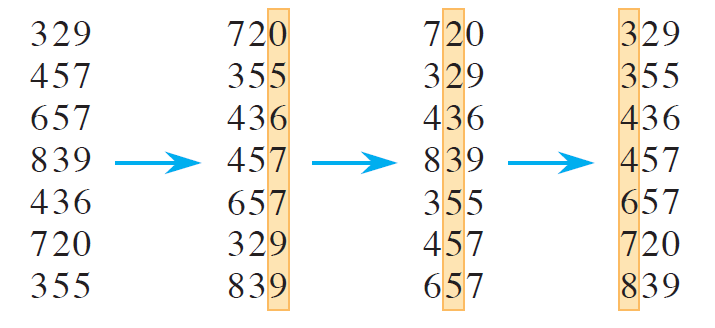
\includegraphics[scale=0.5]{./Immagini_EX/RadixSort.png}
    \caption*{Esempio di ordinamento}
\end{figure}

\noindent Radix Sort, per funzionare correttamente, richiede un algoritmo di ordinamento stabile per l'ordinamento delle singole cifre (o caratteri, a seconda del caso).\bigbreak
\noindent Solitamente, come algoritmo sottostante viene utilizzato Counting Sort, il quale, però, nella sua versione tradizionale non è stabile. Infatti, in presenza di chiavi uguali, Counting Sort potrebbe modificare l'ordine relativo degli elementi rispetto all'array di input.\bigbreak
\noindent Per garantire la stabilità, è sufficiente iterare l'array di input in ordine inverso durante la fase di costruzione dell'array di output. In questo modo, quando più elementi hanno la stessa chiave, essi verranno copiati nell'output nello stesso ordine in cui compaiono nell'input, preservando così la stabilità dell'ordinamento.



\subsubsection{Analisi delle complessità}
\begin{itemize}
    \item \textbf{Caso ottimo: }Le condizioni del caso ottimo di RadixSort sono:
    \begin{itemize}
        \item \textit{d} piccolo;
        \item $k < n$.
    \end{itemize}
    La complessità rimane $\Theta(d(n + k))$, tuttavia, con valori di $d$ e $k$ costanti si ottiene un $\Theta(n)$.
    \item \textbf{Caso pessimo: }Il caso peggiore si verifica nelle condizioni di:
    \begin{itemize}
        \item $d$ elevato (numeri molto grandi);
        \item $k \geq n$ (rende CountingSort inefficiente).
    \end{itemize}
    La complessità resta $\mathcal{O}(d(n + k))$, ma può degenerare fino a diventare $\mathcal{O}(n\cdot log(n))$
    \item \textbf{Caso medio: }Considerando \textit{n} elementi da ordinare, ciascuno composto da \textit{d} cifre, e assumendo che ogni cifra possa assumere al più \textit{k} valori distinti, Radix Sort ha una complessità asintotica pari a $\Theta(d(n + k))$.\\
    Tuttavia, ciò è valido solo se l'algoritmo utilizzato per ordinare le singole cifre (come Counting Sort) ha complessità $\Theta(n + k)$, ovvero è lineare rispetto al numero di elementi e all'ampiezza del dominio delle cifre.
\end{itemize}

\subsubsection{Motivazioni della scelta}
É stato scelto RadixSort come quarto algoritmo a scelta per il suo approccio innovativo e diverso rispetto agli altri algoritmi selezionati, offrendo una prospettiva di confronto interessante.\\
Oltre a ciò, si tratta di un algoritmo utile e applicato in vari contesti reali.\bigbreak
\noindent RadixSort, inoltre, varia la efficienza in base all'algoritmo di ordinamento sottostante, il quale, nel nostro caso countingSort, deve essere stabile per preservare l'ordinamento parziale ottenuto nelle iterazioni precedenti. La stabilità di CountingSort garantisce che elementi con la stessa cifra nella posizione corrente mantengano l'ordine relativo stabilito nelle cifre precedenti, condizione essenziale per la correttezza dell'algoritmo. L'uso di CountingSort come subroutine conferisce a RadixSort una complessità lineare $\mathcal{O}(d \cdot n)$ poiché $k = 10$ (base fissa) è costante, rendendolo particolarmente efficiente per chiavi numeriche con un numero limitato di cifre $d$.

\subsubsection{Codice}
\begin{lstlisting}[style=mycodestyle, language=Python]
def RadixSort(arr):
    radix_array = [[], [], [], [], [], [], [], [], [], []]  # array delle cifre
    max_val = max(arr)  # assegno il valore massimo dell'array
    exp = 1 

    while (max_val // exp) > 0:
        while len(arr) > 0:
            val = arr.pop()
            radix_index = (val // exp) % 10
            radix_array[radix_index].append(val)

        for bucket in radix_array:
            while len(bucket) > 0:
                val = bucket.pop()
                arr.append(val)

        exp *= 10
\end{lstlisting}

\subsubsection*{Funzionamento del codice}
\begin{enumerate}

\item \textbf{Funzione GetMax(A):} Lo scopo è trovare il valore massimo nell'array. A è l'array di elementi. Inizializza \texttt{max} con il primo elemento; scorre tutti gli elementi dall'indice 1 alla fine; se \texttt{A[i] > max}, aggiorna \texttt{max} con \texttt{A[i]}. Restituisce il valore massimo. Costo $\mathcal{O}(n)$.

\item \textbf{Funzione CountingSortForRadix(A, exp):} Lo scopo è ordinare l'array in base a una specifica cifra. A è l'array da ordinare, \texttt{exp} è l'esponente che definisce la cifra (1, 10, 100...). Inizializza un array di output \texttt{B} di dimensione \texttt{n}; un array di conteggio \texttt{C} di dimensione 10 (base) inizializzato a zero; conta le occorrenze di ogni cifra in \texttt{(A[i] / exp) \% 10} in \texttt{C}; modifica \texttt{C} in somme cumulative; costruisce \texttt{B} partendo dalla fine di \texttt{A} per stabilità; copia \texttt{B} in \texttt{A}. Costo $\mathcal{O}(n + k)$ con $k=10$.

\item \textbf{Funzione RadixSort(A):} Lo scopo è ordinare l'array elaborando le cifre dalla meno alla più significativa. A è l'array da ordinare. Trova \texttt{m = GetMax(A)}; per ogni \texttt{exp} (da 1, a 10, a 100... finché \texttt{m/exp > 0}), applica \texttt{CountingSortForRadix(A, exp)}. All'ultima iterazione, l'array è ordinato. Costo $\mathcal{O}(d \cdot (n + k))$ dove $d$ è il numero di cifre.

\end{enumerate}


\section{Misurazioni}

\subsection{Analisi delle Prestazioni al Variare della Dimensione dell'Array (Scala Lineare e Logaritmica)}
\begin{figure}[H]
    \centering
    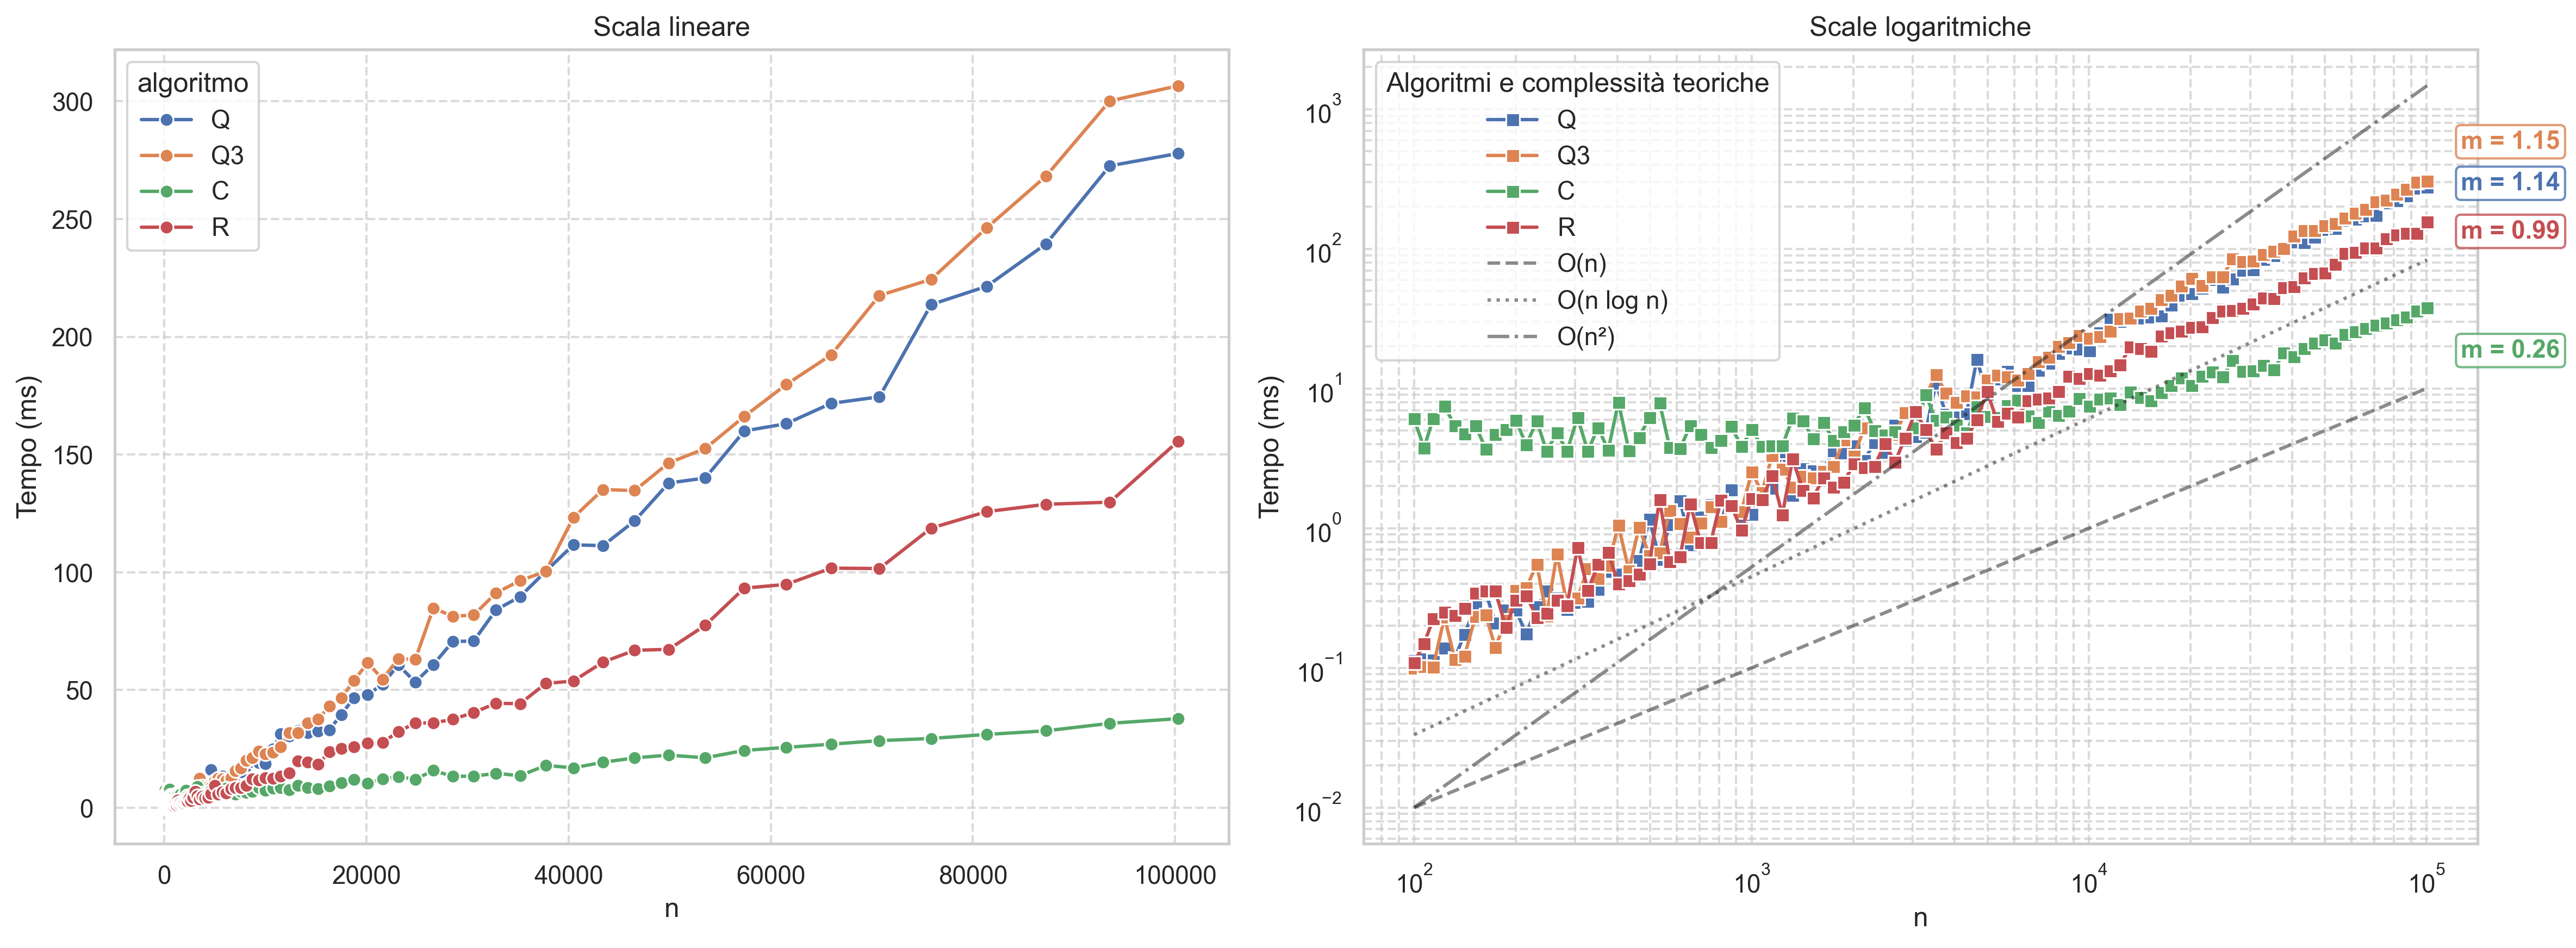
\includegraphics[width=\textwidth]{Immagini/confronto_DEFINITIVO.png}
    \caption*{\textbf{Tempo vs \(n\) (scala lineare).} Tempo medio di esecuzione al variare di \(n\) (con \(m=100\,000\) costante).}
    \label{fig:grafico}
\end{figure}

\subsubsection{Descrizione e obiettivo}
\label{descrizione-obiettivo}
Questo grafico mostra il tempo medio di esecuzione in funzione della dimensione dell'input \(n\) con \(m\) fissato a 100000. Lo scopo è confrontare i tempi assoluti rilevati e visualizzare l'overhead pratico degli algoritmi.

\paragraph{Osservazioni sul grafico lineare}
\begin{itemize}
  \item In ordine dal meno efficiente al più efficiente: QuickSort, QuickSort3Way, RadixSort, CountingSort.
  \item Si nota che per input piccoli (array con $n$ piccolo) hanno efficienza simile. 
  \item Con input grandi notiamo che tutti e 4 gli algoritmi crescono quasi linearmente senza pendenze altalenanti.
  \item Al tempo $t = 100$ (input circa $38.000$), QuickSort e QuickSort3Way si sovrappongono con stesso tempo di esecuzione. In generale hanno andamento simile.
  \item CountingSort invece presenta una crescita molto lenta, mantenendo un'ottima efficienza anche per input molto grandi.
\end{itemize}

\paragraph{Osservazioni sul grafico logaritmico}
\begin{itemize}
  \item Per QuickSort e QuickSort3Way abbiamo costo medio $O(n \log n)$ (pendenze 1.14 e 1.15, rispettivamente)
  \item Per RadixSort costo medio $O(d \cdot n)$ (pendenza 0.99)
  \item Per CountingSort costo medio $O(n + k)$ (pendenza 0.26, apparentemente costante)
  \item Le distribuzioni di QuickSort e QuickSort3Way sono quasi sovrapposte, mentre RadixSort è molto vicina alle due
  \item CountingSort mostra un andamento quasi costante fino a $n \approx 10^3$-$10^4$, per poi aumentare moderatamente restando comunque inferiore agli altri
\end{itemize}

\subsection{Analisi delle Prestazioni al Variare del Range di Valori presenti nell'array (Scala Lineare e Logaritmica)}
\begin{figure}[H]
    \centering
    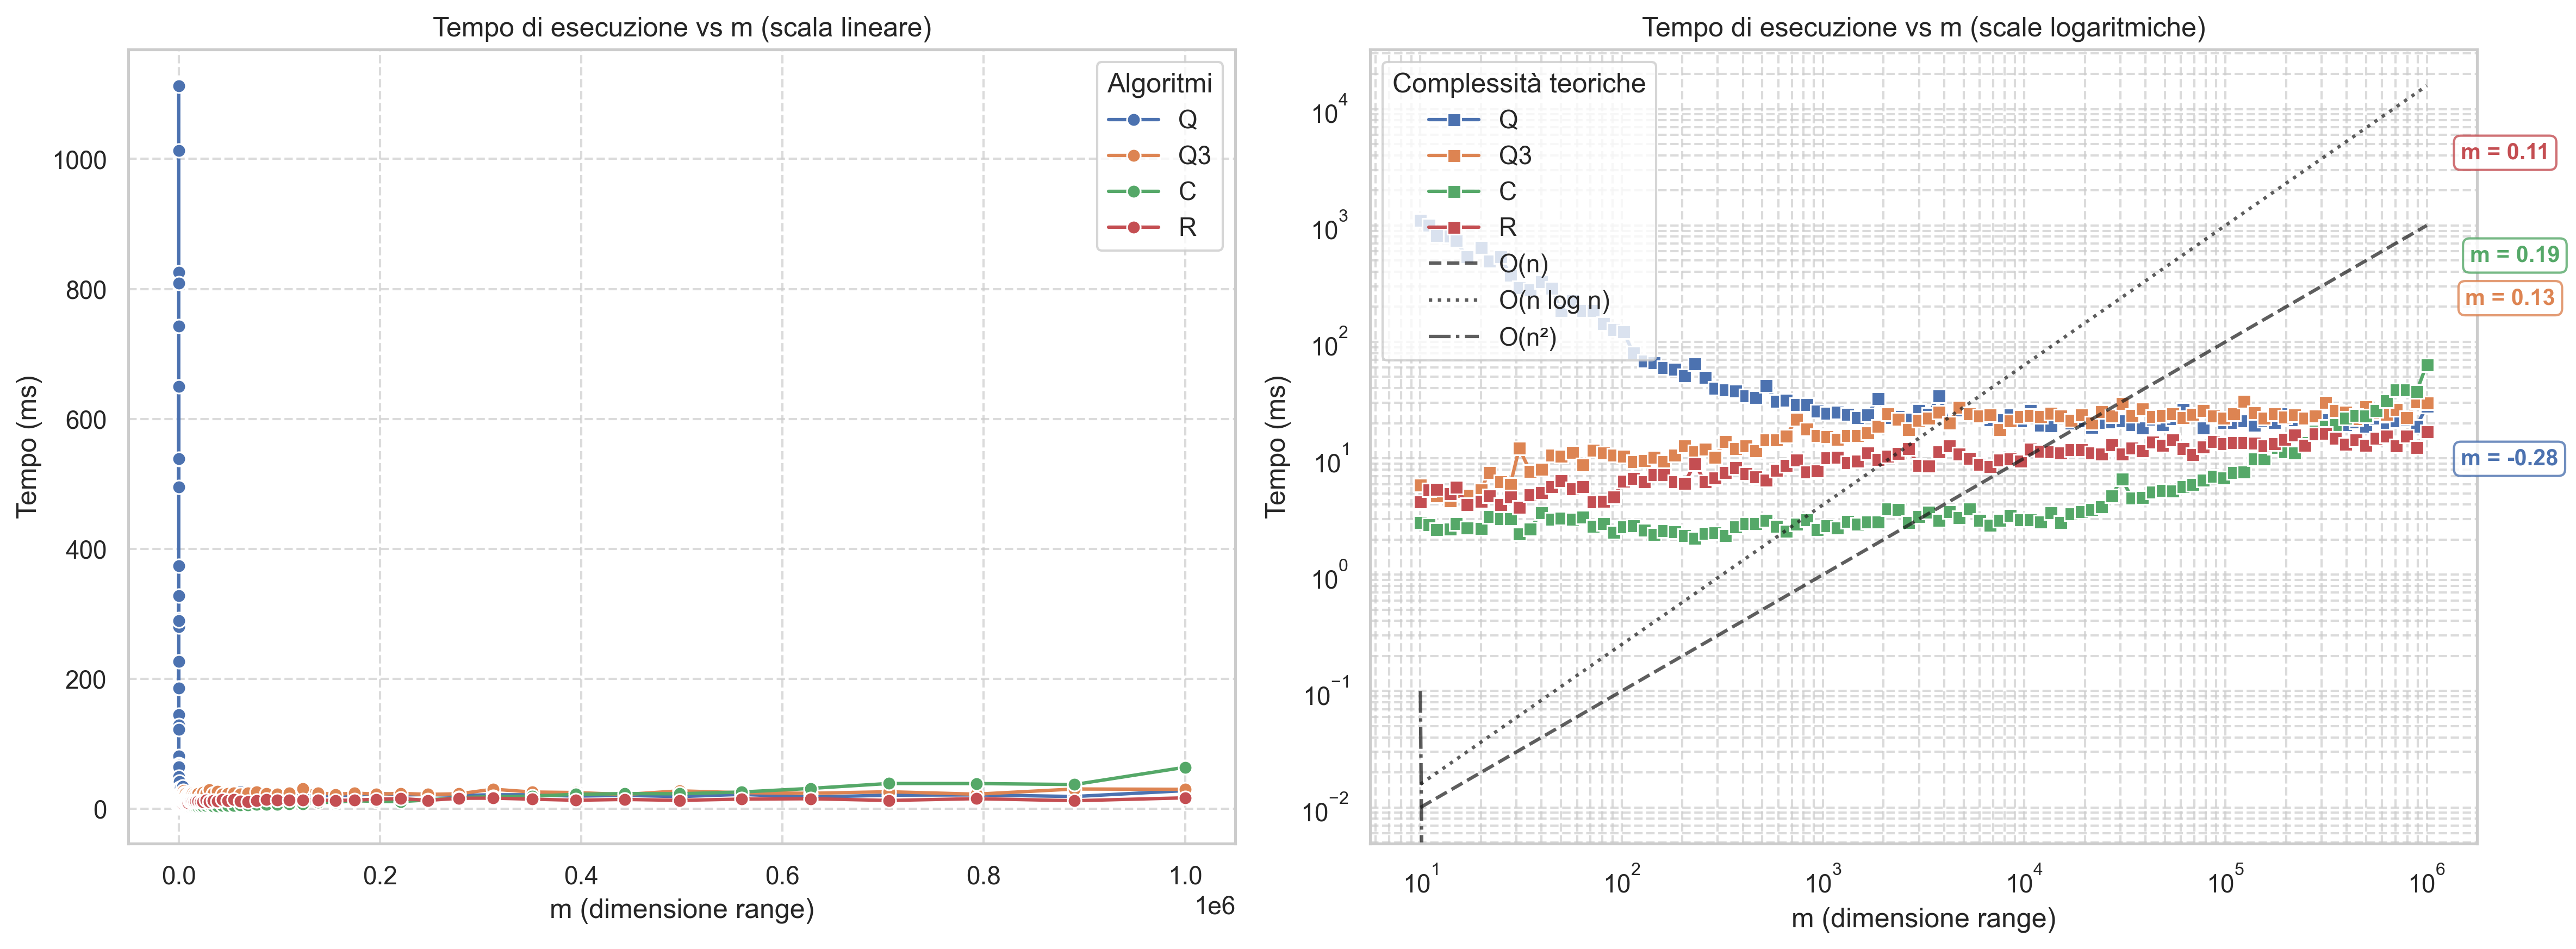
\includegraphics[width=\textwidth]{Immagini/confronto_algoritmi_m_variabile_DEF.png}
    \caption*{\textbf{Tempo vs \(n\) (scala lineare).} Tempo medio di esecuzione al variare di \(m\) (con \(n=10\,000\) costante).}
    \label{fig:grafico}
\end{figure}

\subsubsection{Descrizione e obiettivo}
\label{descrizione-obiettivo}
Questo grafico mostra il tempo medio di esecuzione in funzione della dimensione del range di valori \(m\) con \(n\) fissato a 10000. Lo scopo è confrontare i tempi assoluti rilevati e visualizzare l'overhead pratico degli algoritmi.

\paragraph{Osservazioni sul grafico lineare}
\begin{itemize}
  \item Notiamo come l'andamento per CountingSort sia lineare, all'aumentare del range di valori il suo tempo di esecuzione aumenta rispetto a quello degli altri due algoritmi;
  \item Per RadixSort e QuickSort3Way abbiamo un andamento simile e appiattito, per il primo algoritmo l'osservazione rispecchia la sua complessità lineare;
  \item Importante è notare anche come viene QuickSort, per cui abbiamo una retta praticamente verticale, questo può essere dovuto al fatto che il tempo medio di esecuzione dell'algoritmo non dipenda dal range di valori.
\end{itemize}

\paragraph{Osservazioni sul grafico logaritmico}
\begin{itemize}
  \item Possiamo notare che il tempo medio di esecuzione di QuickSort migliora man mano che il range m di valori viene incrementato;
  \item Gli andamenti degli altri tre algoritmi è molto simile con l'unica differenza per CountingSort il cui tempo medio di esecuzione aumenta per valori di un range molto elevato $(10^6)$, gli andamenti di RadixSort e QuickSort3Way sono quasi uguali sennonchè RadixSort, in termini
  di tempo medio di esecuzione, è leggermente più efficiente.
  \item QuickSort: $m=-0.28$, all'aumentare del range di valori il tempo diminuisce, il che è un comportamento particolare. 
  (può essere normale se consideriamo che costo medio $O(n \log n)$, e il fatto che magari la scelta del pivot è ottima con l'aumentare della varietà del range di valori)
  \item RadixSort: $m=0.11$, crescita lenta, coerente con la complessità $d \cdot O(n)$;
  \item CountingSort: $m=0.19$, crescita lenta, non molto coerente dato che ci aspetteremmo una complessità lineare $O(n + k) = O(n) \quad \text{se} \quad k = O(n)$;
  \item QuickSort3Way: $m=0.13$, crescita lenta, coerente con la complessità $O(n \log n)$.
\end{itemize}

\section{Conclusioni}

\end{document}